\subsection{Loop antenna with gap}\label{sec:loop_gap_sim}
\subsubsection{Setup and geometrical analysis}\label{sec:loop_gap_setup}
\FloatBarrier
\begin{figure}[h]

\end{figure}
\begin{figure}

\end{figure}

\begin{figure}[htbp]
	\centering
	\begin{subfigure}[t]{0.48\textwidth}
		\centering
		\includegraphics[width=1\linewidth]{content/img/gap_loop_antenna_fields}
		\caption{Electric near-field intensity}
		\label{fig:gaploopantennafields}
	\end{subfigure}
	\hfill
	\begin{subfigure}[t]{0.48\textwidth}
		\centering
		\includegraphics[width=1\linewidth]{content/img/gapped_loop_antenna}
		\caption{Geometry of loop antenna with gap}
		\label{fig:gappedloopantenna}
	\end{subfigure}
	
	\caption{Geometry of the loop antenna with a gap in the return path inserted in the TEM cell. The gap height is exaggerated for demonstration purposes.}
	\label{fig:example}
\end{figure}

The geometry of the loop antenna with a gap is similar to that of the loop antenna discussed in \autoref{sec:loop_sim}. It is electrically short for frequencies up to 4.69\,GHz. A gap with a height of $10\,\upmu\mathrm{m}$ is introduced in the return path, as shown in \autoref{fig:gappedloopantenna}. The gap is intentionally kept small to emphasize specific coupling mechanics and to demonstrate the consistency of antenna analysis with the framework developed in this thesis, although such a small gap would be hard to implement in a physical antenna. Furthermore, manual mesh refinement is necessary around the gap region, as well as the feedpoint and the curved surfaces, as discussed in \autoref{sec:mesh}.	

The magnetic coupling is determined with \crefrange{eqn:e_a_closed_int}{eqn:e_b_closed_int}, just as is the case for the normal loop antenna. However, considering the gap region leads to 

\begin{equation}
	-\oint_C \boldsymbol{\tau} I(l) \cdot\mathbf{e}_n^\pm  dl= -\int_\text{wire} \boldsymbol{\tau} I_\text{wire}(l) \cdot\mathbf{e}_n^\pm  dl -\int_\text{gap} \boldsymbol{\tau} I_\text{gap}(l) \cdot\mathbf{e}_n^\pm  dl.
\end{equation}

The electric current across the gap is $I_\mathrm{gap}=0\,\mathrm{A}$, while the current in the antenna wire $I_\mathrm{wire}$ is significantly reduced due to the interrupted current path. Consequently, the magnetic coupling between the loop antenna with a gap and the TEM cell is expected to be weaker than that of the loop antenna without a gap, but still more present than the monopole antenna discussed in \autoref{sec:monopole}. Furthermore, reducing the gap height increases magnetic coupling and the magnitude of the magnetic dipole moment $\mathbf{m}_m$, attributable to the correlated increase of $I_\mathrm{wire}$.

The conductors adjacent to the gap behave as capacitors plates, accumulating charges on both either side. According to \crefrange{eqn:charges_a}{eqn:charges_b}, these accumulated charges lead to electric coupling with the septum. A smaller gap height increases the amount of accumulated charges, and consequently leads to an increase in the electric dipole moment $\mathbf{m}_e$. Lastly, the absence of a conductive return path for the current leads to expect capacitive behavior of this electrically small antenna, similar to the monopole antenna analyzed in \autoref{sec:monopole}.

\todo[inline]{Ideas: see LaTeX comments}

%\todo[inline]{TODO: Some sources state that electrically small antennas must be either strongly capacitive or inductive. This would mean, that small antennas can always be represented by the same model: Either dominating electric dipole moment in the capacitive antenna case, with a non-linear behavior of the high frequencies, or a magnetic dipole moment with the same property in the inductive antenna case. The frequency, at which the non-linearities occur, depend on the amount of capacitance or inductance, i.e. the Q-factor. A high Q-factor leads to non-linearities in lower cut-off frequencies, and a low Q-factor increases the cut-off frequency. A capacitive antenna with low impedance has a high Q-factor. A inductive antenna with high impedance has a high Q-factor. This can practically be read from the impedance graphs. Can a relation between the impedance/Q-factor and a ``cut-off frequency'' of the dipole moments be established?}
%
%\todo[inline]{TODO: A little thought experiment on the gapped loop antenna demonstrates why this is the case: If the magnetic dipole moment shall be increased in this antenna, the height of the gap can be decreased to increase the current flow and therefore the magnetic coupling. Ironically, this also increases the amount of charges accumulating on the boundaries of the gap, therefore increasing the electric coupling and capacitive behavior. The capacitive behavior can therefore not change, unless the gap is completely removed. Also, the decrease in gap leads to larger total energy transfer and a higher Q-factor. I suspect, that a high Q-factor of an antenna leads to high energy transfer. This would make sense, because a high Q-factor indicates increased near-field intensities, that would naturally couple with the tem cell. A simulation showing the dipole moments for different gap heights over the frequency would support this claim.}

\subsubsection{Equivalent dipole moments}

The equivalent dipole moments of the loop antenna with gap are shown in \autoref{fig:gappedloopmoments}, where the electric dipole moment $\mathbf{m}_e$ is larger than the magnetic dipole moment $\mathbf{m}_m$. The dipole moments behave non-linearly over the frequency. 

\begin{figure}[htbp]
	\centering
	
	\begin{subfigure}[t]{0.5\textwidth}
		\centering
		\includegraphics[width=1\linewidth]{content/img/gapped_loop_moments}
		\caption{Equivalent dipole moments over frequency}
		\label{fig:gappedloopmoments}
	\end{subfigure}
	\hfill
	\begin{subfigure}[t]{0.48\textwidth}
		\centering
		\includegraphics[width=1\linewidth]{content/img/gapped_loop_phase}
		\caption{Phase of the power at each output port}
		\label{fig:gappedloopphase}
	\end{subfigure}
	
	\caption{The equivalent dipole moments of the loop antenna with a gap, where the electric dipole moment $\mathbf{m}_\mathrm{e}$ is weighted with $Z_0$ to enable comparison with $\mathbf{m}_\mathrm{m}$. The phases of the powers at output ports 1 and 2 are derived from the S-parameters, as discussed in \cref{sec:s-param-data}. The analysis specifically focuses on the phase shift between the two ports, which provides information about the presence of $\mathbf{m}_\mathrm{m}$ and $\mathbf{m}_\mathrm{e}$, as investigated in \cref{sec:equ-dip-mom}.}
	\label{fig:example}
\end{figure}

\autoref{fig:gappedloopcompmomentsgapsweep} demonstrates the effect of the gap height on the dipole moment behavior. As discussed in \autoref{sec:loop_gap_setup}, the reduction of the gap height leads to an increase of both dipole moments, $\mathbf{m}_\mathrm{e}$ and $\mathbf{m}_\mathrm{m}$. Their magnitudes correlate with the output power, as shown in \autoref{fig:gappedloopcomppowergapsweep}.

\begin{figure}[htbp]
	\centering
	\begin{subfigure}[b]{0.48\textwidth}
		\centering
		\includegraphics[width=1\linewidth]{content/img/gapped_loop_comp_moments_gap_sweep}
		\caption{Equivalent dipole moments}
		\label{fig:gappedloopcompmomentsgapsweep}
	\end{subfigure}
	\hfill
	\begin{subfigure}[b]{0.48\textwidth}
		\centering
		\includegraphics[width=1\linewidth]{content/img/gapped_loop_comp_power_gap_sweep}
		\caption{Output power}
		\label{fig:gappedloopcomppowergapsweep}
	\end{subfigure}
	
	\caption{Comparison of dipole moments, where the electric dipole moment $\mathbf{m}_\mathrm{e}$ is weighted with $Z_0$ to enable comparison with $\mathbf{m}_\mathrm{m}$, and output power for different gap heights in the loop antenna.}
	\label{fig:example}
\end{figure}

An increase in gap height reduces the non-linearities in $\mathbf{m}_\mathrm{e}$ and $\mathbf{m}_\mathrm{m}$. The voltage drop across the gap and the charge accumulation remains stabler over frequency. A small gap leads to both an increase in current and inductance, therefore creating a large voltage drop and influencing $\mathbf{m}_\mathrm{e}$ and $\mathbf{m}_\mathrm{m}$.

\subsubsection{Electrical characteristics}

%\begin{figure}[htbp]
%	\centering
%	\begin{subfigure}[b]{0.48\textwidth}
%		\centering
%		\includegraphics[width=1\linewidth]{content/img/gapped_loop_opower}
%		\caption{Output electric field and power}
%		\label{fig:gappedloopopower}
%	\end{subfigure}
%	\hfill
%	\begin{subfigure}[b]{0.48\textwidth}
%		\centering
%		\includegraphics[width=1\linewidth]{content/img/gapped_loop_voltage}
%		\caption{Peak feed voltage}
%		\label{fig:gappedloopvoltage}
%	\end{subfigure}
%	
%	\caption{Electric field and power at the TEM cell's output port, and the peak feed voltage of the antenna.}
%	\label{fig:example}
%\end{figure}



%\begin{figure}[htbp]
%	\centering
%	\begin{subfigure}[b]{0.48\textwidth}
%		\centering
%		\includegraphics[width=1\linewidth]{content/img/gapped_loop_current}
%		\caption{RMS feed current.}
%		\label{fig:gappedloopcurrent}
%	\end{subfigure}
%	\hfill
%	\begin{subfigure}[b]{0.48\textwidth}
%		\centering
%		\includegraphics[width=1\linewidth]{content/img/gapped_loop_imp}
%		\caption{Magnitude and phase of impedance}
%		\label{fig:gappedloopimp}
%	\end{subfigure}
%	\label{fig:example}
%\end{figure}


The impedance of the loop antenna with gap is capacitive, shown in \autoref{fig:gappedloopimp},
The inductance of this antenna is not negligible, opposed to the case of the monopole antenna in \autoref{sec:monopole}. This causes a significant magnitude of $\mathbf{m}_\mathrm{m}$ in \autoref{fig:gappedloopmoments} and a stronger decline in impedance magnitude of the loop antenna with gap, compared to the monopole antenna's impedance, demonstrated in \autoref{fig:monopoleimp}. 

The feedpoint voltage decreases more rapidly over frequency compared to that of the monopole antenna, see \crefrange{fig:gap-loop-voltage-current}{fig:loopfeedreturncurrent}. This behavior is a direct result of increased induced voltage, which correlates with the pronounced magnetic dipole moment $\mathbf{m}_m$, according to \autoref{eqn:m_v}. Furthermore, the feed current increases more slowly, resulting in a slower growth of the electric dipole moment $\mathbf{m}_e$ with frequency, according to \autoref{eqn:me_i}. The magnitude of $\mathbf{m}_e$ is additionally smaller than that of the monopole in \autoref{fig:dipolemomentsmonopolewide}. 

\begin{figure}[htbp]
	\centering
	\begin{subfigure}[b]{0.48\textwidth}
		\centering
		\includegraphics[width=1\linewidth]{content/img/gap-loop-voltage-current}
		\caption{Voltage and current across feedpoint}
		\label{fig:gap-loop-voltage-current}
	\end{subfigure}
	\hfill
	\begin{subfigure}[b]{0.48\textwidth}
		\centering
		\includegraphics[width=1\linewidth]{content/img/gapped_loop_imp}
		\caption{Magnitude and phase of impedance}
		\label{fig:gappedloopimp}
	\end{subfigure}
	\caption{The voltage and current across the feedpoint, together with the related impedance of the loop antenna with gap.}
	\label{fig:example}
\end{figure}
